% ============================================================
% UGA-Themed Beamer Presentation
% Love of Variety, Habit Formation, and Dynamic Advertising
%
% Compile with:
%   pdflatex presentation.tex
% ============================================================

\documentclass[aspectratio=169,professionalfonts]{beamer}

% ---------- COLORS ----------
\usepackage{xcolor}
\definecolor{UGARed}{HTML}{BA0C2F}
\definecolor{UGABlack}{HTML}{000000}
\definecolor{UGAGray}{HTML}{8A8D8F}

% ---------- THEME ----------
\usetheme{default}
\useinnertheme{circles}
\useoutertheme[subsection=false]{miniframes}
\usefonttheme{professionalfonts}
\setbeamertemplate{navigation symbols}{}

% Head/foot colors
\setbeamercolor{subsection in head/foot}{fg=white, bg=UGARed}
\setbeamercolor{headline}{fg=white, bg=UGARed}
\setbeamercolor{section in head/foot}{fg=white, bg=UGARed}
\setbeamercolor{section in head/foot shaded}{fg=white, bg=white}
\setbeamercolor{footline}{bg=UGABlack, fg=white}
\setbeamercolor{frametitle}{fg=UGABlack}
\setbeamercolor{title}{fg=UGABlack}
\setbeamercolor{normal text}{fg=UGABlack}
\setbeamercolor{structure}{fg=UGARed}

% Headline
\setbeamertemplate{headline}{
  \begin{beamercolorbox}[wd=\paperwidth,ht=2.5ex,dp=1.125ex]{headline}
    \insertsectionnavigationhorizontal{\paperwidth}{}{}
  \end{beamercolorbox}
}

% Footline
\setbeamertemplate{footline}{%
  \leavevmode%
  \hbox{%
    \begin{beamercolorbox}[wd=\paperwidth,ht=2.5ex,dp=1ex,leftskip=1em,rightskip=1em]{footline}%
      \ifnum\theframenumber=0\relax\else%
        \insertshortauthor{} \hfill \insertframenumber/\inserttotalframenumber%
      \fi%
    \end{beamercolorbox}}%
}

% ---------- PACKAGES ----------
\usepackage{appendixnumberbeamer}
\usepackage{amsmath, amssymb, mathtools}
\usepackage{booktabs}
\usepackage{graphicx}
\usepackage{hyperref}
\usepackage{tcolorbox}

% ---------- METADATA ----------
\title[Love of Variety \& Dynamic Advertising]{%
    Love of Variety and Dynamic Advertising}
\subtitle{}
\author[T. Mason]{Tate Mason}
\institute[UGA]{John Munro Godfrey Sr.\ Dept.\ of Economics \\ University of Georgia}
\date{\today}

% ---------- AUTO-AGENDA ----------
\AtBeginSection[]{
  \begin{frame}[noframenumbering]{Roadmap}
    \tableofcontents[currentsection]
  \end{frame}
}

% ---------- MACROS ----------
\newcommand{\E}{\mathbb{E}}
\newcommand{\R}{\mathbb{R}}
\newcommand{\hl}[1]{\textbf{\textcolor{UGARed}{#1}}}
\hypersetup{colorlinks=true, linkcolor=UGARed, urlcolor=UGARed}

% ============================================================
\begin{document}

% ------------------------------------------------------------
% Title
% ------------------------------------------------------------
\begin{frame}[noframenumbering]
  \titlepage
\end{frame}

% ============================================================
\section{Motivation}
% ============================================================

\begin{frame}{Motivation: Data Privacy, Ad Targeting, and Consumer Agency}
  \begin{itemize}
    \item Amazon anti-trust scrutiny
    \begin{itemize}
      \item Amazon accounts for almost $40\%$ of US e-commerce sales (Statista, 2023)
      \item Able to use consumer data to target ads and build market share as both retailer and platform
    \end{itemize}
    \item Consumer agency over data (opt out)
    \begin{itemize}
      \item Apple iOS 14.5 update: $85\%$ opt-out rate upon rollout (Flurry Analytics, 2022)
      \item Facebook ad revenue down \$13bn in 2022 due to app tracking transparency (ATT) policy
    \end{itemize}
  \end{itemize}
  \begin{tcolorbox}[colback=red!5!white, colframe=UGARed, title=\textbf{Key Concern}]
    How do data privacy policies that limit firms' ability to target ads based on consumer data impact consumer welfare and firms' incentives to invest in product quality and advertising?
  \end{tcolorbox}
\end{frame}

\begin{frame}{Why Does Variety Matter?}
  \begin{tcolorbox}[colback=red!5!white, colframe=UGARed, title=\textbf{Research Question}]
    How do consumer preferences for variety impact the firms' targeting strategy and what are the welfare implications of data privacy policies that limit ad targeting?
  \end{tcolorbox}
  \begin{itemize}
    \item Understanding the role of variety-seeking is valuable for modeling consumer behavior and evaluating the impact of data privacy policies on both consumers and firms.
    \item Canonical logit models ignore consumer preferences for variety, which are
          empirically important 
    \item These preferences may shape consumer switching behavior, which in turn
          shapes firms' incentives to strategically target ads and promotions (i.e. to encourage switch to a higher markup product)
  \end{itemize}
\end{frame}

\begin{frame}{What This Paper Does (So Far)}
  \begin{enumerate}
    \item \hl{Model:} Dynamic discrete choice model of consumer behavior with love of variety and strategic advertising by firms
    \vspace{4pt}
    \item \hl{Simulation:} Characterize consumer and firm behavior
          across preference regimes and advertising
          specifications
    \vspace{4pt}
    \item \hl{Estimation (coming):} Bring model to Nielsen scanner data
          to recover structural parameters
    \vspace{4pt}
    \item \hl{Counterfactuals (coming):} Study advertising targeting policy and
          welfare implications
  \end{enumerate}
  \vspace{6pt}
  \textbf{Today's talk:} Consumer demand function + simulation results
\end{frame}

\begin{frame}{Literature Connections}
  \begin{columns}[T]
    \begin{column}{0.48\textwidth}
      \hl{Demand side}
      \begin{itemize}
        \item Lattin (1987): State dependence in consumer choice
        \item Chintagunta (1999): Extension to panel data
        \item Dub\'e, Hitsch, Rossi (2009): Habit formation and switching costs
      \end{itemize}
    \end{column}
    \begin{column}{0.48\textwidth}
      \hl{Advertising / firm side}
      \begin{itemize}
        \item Shaffer and Zhang (1995): Theoretical basis for ad targeting in a two-period model
        \item Erdem \& Keane (1996): Learning dynamics
        \item Zhang, Choi, Cheng (2025): Updated targeting game
      \end{itemize}
    \end{column}
  \end{columns}

  \vspace{1pt}
  \begin{tcolorbox}[colback=red!5!white, colframe=UGARed, title=\textbf{Contribution}]
    Unite the demand and supply side literatures by modeling consumer preferences for variety in a dynamic discrete choice framework with strategic advertising.
  \end{tcolorbox}
\end{frame}

% ============================================================
\section{Model}
% ============================================================

\begin{frame}{Consumer's Problem}
  Consumer $i$ chooses product $j$ in period $t$ to maximize:
  \begin{equation*}
    U_{ijt} = \underbrace{\beta_{ij} X_{jt}}_{\text{characteristic component}}
              + \underbrace{\gamma_i \log(1 + \Sigma_{ijt}^2)}_{\text{novelty component}}
              - \underbrace{\alpha \, p_{jt} (1-a_{jt})}_{\text{ad-adjusted price}}
              + \xi_{j} + \varepsilon_{ijt}
  \end{equation*}
  \begin{itemize}
    \item where $\Sigma_{ijt} = X_{jt} - \theta_{it}$ is the deviation of product $j$'s characteristic from consumer $i$'s previously chosen characteristics $\theta_{it}$ in period $t$.
    \item at the moment, $\theta_{it} = \frac{1}{t}\sum_{s=1}^{t-1} X_{js}$, or the mean of previously chosen product characteristics.
  \end{itemize}
  \vspace{8pt}
  \begin{columns}[T]
    \begin{column}{0.48\textwidth}
      \hl{Key parameters:}
      \begin{itemize}
        \item $\beta_i > 0$: quality
        \item $\gamma_i > 0$: variety-seeking
      \end{itemize}
    \end{column}
    \begin{column}{0.48\textwidth}
      \hl{Choice probability (MNL):}
      \begin{equation*}
        P_{ijt} = \frac{e^{U_{ijt}}}{1 + \sum_{k} e^{U_{ikt}}}
      \end{equation*}
      Follows from $\varepsilon_{ijt} \sim \text{Gumbel}(0,1)$
    \end{column}
  \end{columns}
\end{frame}

\begin{frame}{State Variable: History of Choices}
  \begin{tcolorbox}[colback=red!5!white, colframe=UGARed, title=\textbf{History of Choices $\theta_{it}$}]
    \[
    \theta_{it} = f(\{X_{js}\}_{s < t}) = \frac{1}{t}\sum_{s=1}^{t-1} X_{js}
    \]

    The consumer's history is summarized by the mean of previously chosen product characteristics.
  \end{tcolorbox}

  \vspace{6pt}
  \hl{Simulation design:}
  \begin{itemize}
    \item \textbf{Initial state:} Simulate $T_{\text{prior}} = 5$ pre-sample
          periods, choose products from $J \in [1,2,3,4,5]$ to generate an experience-based
          prior.
  \end{itemize}
\end{frame}

%\begin{frame}{Firm's Problem}
%  \hl{Firm $j$ solves a dynamic program:}
%  \[
%    V_j(t; \Sigma_{jt}, \lambda_t(\gamma_i)) = \max_{a \in \{0,1\}}
%    \left\{ \pi_{jt}(a) + \beta_{df} \, \E\bigl[V_j(t{+}1;\cdot)\bigr] \right\}
%  \]
%
%  \vspace{4pt}
%  \hl{Per-period profit:}
%  \[
%    \pi_{jt}(a) = s_{jt}(p - mc) - \mu \, a
%  \]
%
%  \vspace{4pt}
%  \hl{Two advertising specifications:}
%  \begin{itemize}
%    \item \textbf{Fixed:} $a \in \{0, 1\}$ (binary on/off)
%    \item \textbf{Heuristic} $a_t \propto (\bar{X}_{it} - X_{jt-1})^2$
%          --- higher spending when product is far from consumer's mean
%          --- work in progress: not ideal measure of drift
%  \end{itemize}
%
%  \vspace{4pt}
%  Solved via backward induction; firm chooses $a$ to maximize discounted profits (to be completed)
%\end{frame}
% ============================================================
\section{Simulation Design}
% ============================================================

\begin{frame}{Simulation Parameters}
  \begin{table}
    \centering
    \caption{Parameters}
    \begin{tabular}{lll}
      \toprule
      Param. & Value & Description \\
      \midrule
      $T$         & 100             & Periods \\
      $J$         & 5               & Products \\
      $S$         & 1{,}000         & Simulations \\
      $\beta_{ij}$   & 2             & Quality \\
      $\gamma_i$     & $\{6, 9, 12\}$ & Variety-seeking \\
      $\alpha$    & 0               & Price (off) \\
      $\xi_j$     & 0               & Unobserved quality (off) \\
      $\beta_{df}$    & 0             & Discount factor (off) \\
      \bottomrule
    \end{tabular}
  \end{table}
\end{frame}

% ============================================================
\section{Results: Consumer Behavior}
% ============================================================

\begin{frame}{Utility Measurement (No LOV)}
  \begin{tcolorbox}[colback=red!5!white, colframe=UGARed, title=\textbf{Utility Function without LOV}]
    \begin{equation*}
      \hat{U}_{ijt} = \beta_{ij} X_{jt} + \epsilon_{ijt}
    \end{equation*}
  \end{tcolorbox}
  \begin{columns}[T]
    \begin{column}{0.5\textwidth}
      
      \begin{itemize}
        \item Any variation due to $\varepsilon_{ijt}$, not consumer preferences
        \item CCPs are not informative about consumer behavior or firm incentives
        \item Nearly all mass on Product 5, which has the highest quality $X_{jt}$
      \end{itemize}
    \end{column}
    \begin{column}{0.47\textwidth}
      \begin{table}
        \caption{CCPs (No LOV)}
        \begin{tabular}{lc}
          \toprule
          Product & CCP \\
          \midrule
          Product 1     & 0.02\% \\
          Product 2     & 0.54\% \\
          Product 3     & 4.05\% \\
          Product 4     & 22.3\% \\
          Product 5     & 72.0\% \\
          \bottomrule
        \end{tabular}
      \end{table}
    \end{column}
  \end{columns}
\end{frame}

\begin{frame}{Consumer Behavior with LOV}
  \begin{tcolorbox}[colback=red!5!white, colframe=UGARed, title=\textbf{Utility Function with LOV}]
    \begin{equation*}
      \hat{U}_{ijt} = \beta_{ij} X_{jt} + \gamma_i \log(1 + \Sigma_{ijt}^2) + \epsilon_{ijt}
    \end{equation*}
  \end{tcolorbox}
  \begin{itemize}
    \item where $\Sigma_{ijt} = X_{jt} - \theta_{it}$ as before.
    \item Consumer behavior varies significantly across variety specifications.
    \item Higher $\gamma_i$ leads to more switching.
    \item Cross-sectional sorting: consumers with higher $\gamma_i$ are more likely to switch to lower indexed products.
  \end{itemize}
\end{frame}

\begin{frame}{LOV Specification}
  \begin{figure}
    \centering
    \begin{subfigure}
      \centering
      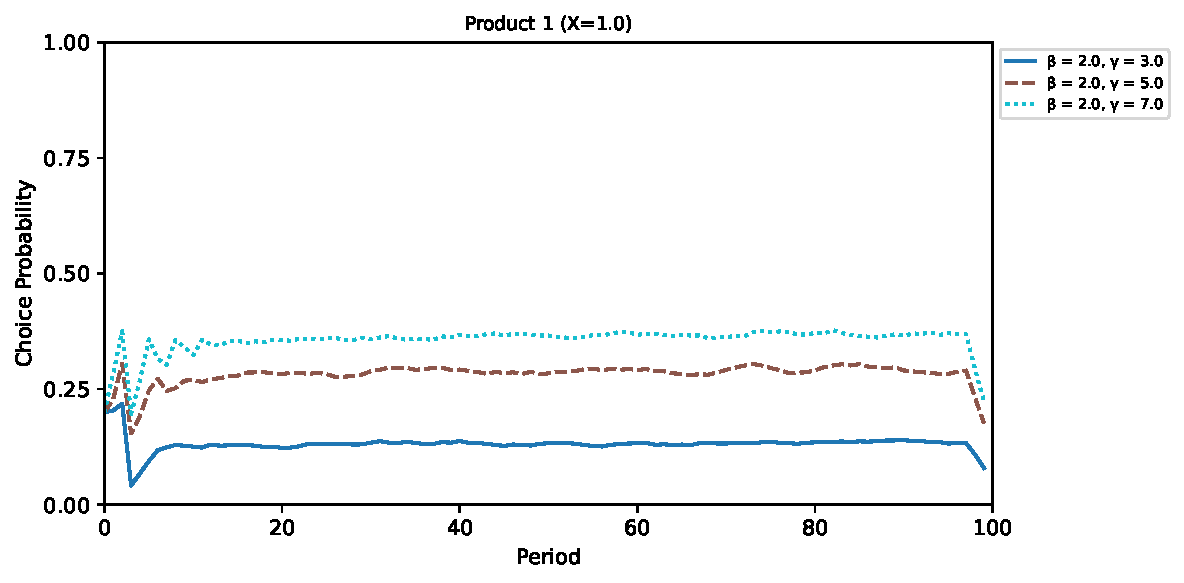
\includegraphics[width=.48\linewidth]{../Output/prior_mean_prob_product_1.pdf}
    \end{subfigure}
    \hfill
    \begin{subfigure}
      \centering
      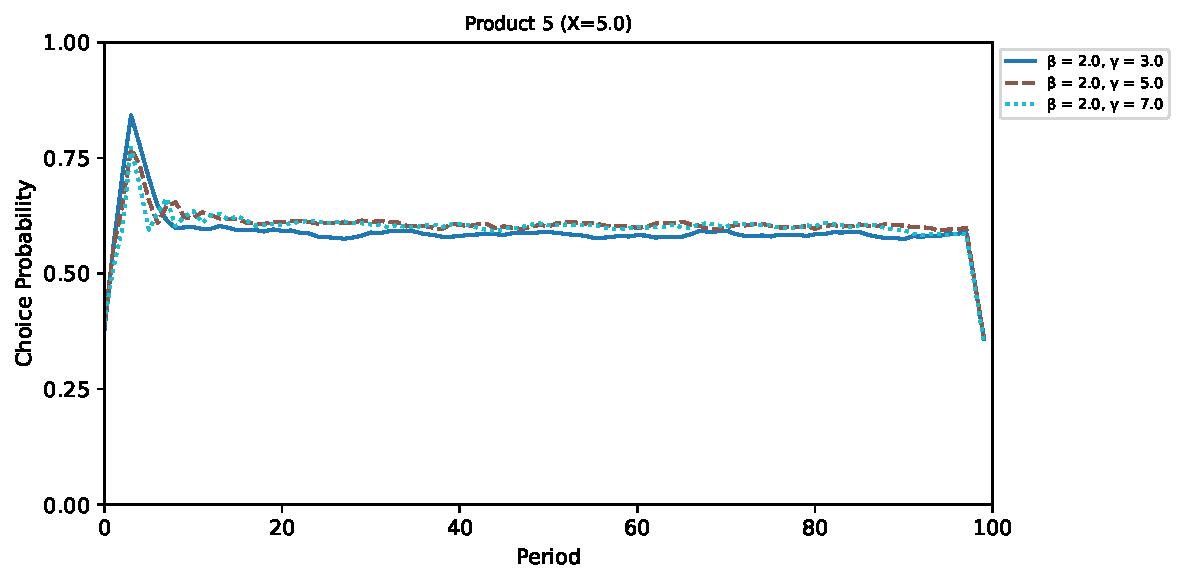
\includegraphics[width=.48\linewidth]{../Output/prior_mean_prob_product_5.pdf}
    \end{subfigure}
    \vspace{4pt}
    \begin{subfigure}
      \centering
      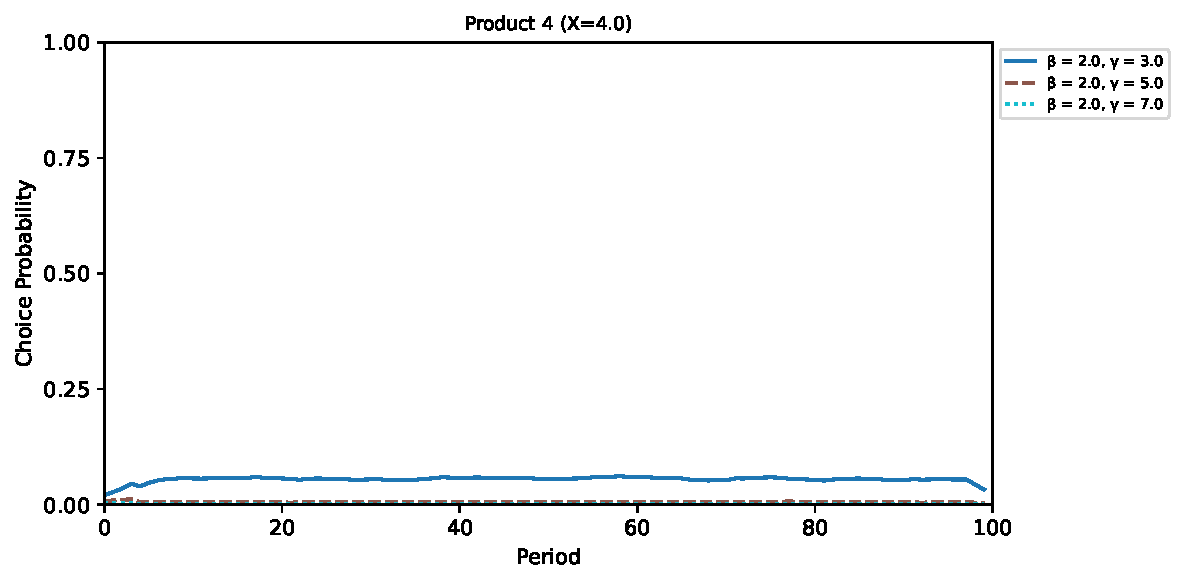
\includegraphics[width=.48\linewidth]{../Output/prior_mean_prob_product_4.pdf}
    \end{subfigure}
  \end{figure}
\end{frame}


% ============================================================
\section{Next Steps}
% ============================================================

\begin{frame}{Road to Estimation}
  \begin{enumerate}
    \item \hl{Multiple consumers} \\
          Extend simulation to $I = 5$ consumers who have heterogeneous $(\beta_i, \gamma_i)$;
          aggregate to market shares

    \vspace{4pt}
    \item \hl{Consumer value function} \\
          Move from reduced-form simulation to solving the full
          dynamic discrete choice with continuation values

    \vspace{4pt}
    \item \hl{Nielsen scanner data} \\
          Match simulated moments to data;
          identify $(\beta_i, \gamma_i)$ using BLP instruments

    \vspace{4pt}
    \item \hl{Firm's Problem} \\
          Ad targeting policy; profit maximization; counterfactuals
  \end{enumerate}
\end{frame}


\begin{frame}{Summary}
  \begin{enumerate}
    \item \hl{Model:} Consumer utility depends on deviation from
          experiences; nests variety-seeking 

    \vspace{4pt}
    \item \hl{History:} Rich behavioral dynamics; greater preference for variety 
          generates cross-sectional sorting

    \vspace{4pt}
    \item \hl{Next:} Multiple consumers, structural estimation,
          Nielsen data
  \end{enumerate}

  \vspace{10pt}
  \centering
  \Large\textbf{Thank you --- questions welcome}
\end{frame}

% ============================================================
% Appendix
% ============================================================
\appendix
\begin{frame}[plain, noframenumbering]
  \centering
  \vspace{2cm}
  {\Large \textbf{Appendix}}
\end{frame}

\begin{frame}{References}
  \begin{thebibliography}{9}
    \footnotesize
    \bibitem{lattin1987}
    Lattin, J. M. (1987). \textit{State dependence in consumer choice}. Journal of Consumer Research, 14(3), 417-431.

    \bibitem{chintagunta1999}
    Chintagunta, P. K. (1999). \textit{Panel data analysis of state dependence and heterogeneity in brand choice behavior}. Journal of Econometrics, 89(1-2), 5-34.

    \bibitem{dube2010}
    Dub\'e, J. P., Hitsch, G. J., \& Rossi, P. E. (2009). \textit{State dependence and alternative explanations for consumer inertia}. NBER Working Paper No. 14912.

    \bibitem{shaffer1995}
    Shaffer, G., \& Zhang, Z. J. (1995). \textit{Competitive advertising in a duopoly}. Marketing Science, 14(3_supplement), G206-G218.

    \bibitem{erdem1996}
    Erdem, T., \& Keane, M. P. (1996). \textit{Decision-making under uncertainty: Capturing dynamic brand choice processes in turbulent consumer goods markets}. Marketing Science, 15(1), 1-20. 

    \bibitem{bronnenberg2012}
    Bronnenberg, B. J., Dub\'e, J. P., \& Gentzkow, M. (2012). \textit{The Evolution of Brand Preferences: Evidence from Consumer Migration}. American Economic Review, 102(6), 2472-2508.

    \bibitem{zhang2025}
    Zhang, J., Choi, J., \& Cheng, S. (2025). \textit{Dynamic advertising targeting: A structural approach}. Marketing Science, 44(1), 1-20.

  \end{thebibliography}
\end{frame}

\begin{frame}{Simulation Algorithm (Consumer)}
  \begin{enumerate}
    \item Draw $\varepsilon_{ijt} \sim \text{Gumbel}(0,1)$ for all $i, j, t$
    \item Initialize $\bar{X}_{i0}$ (set mean or prior mean)
    \item For $t = 1, \ldots, T$:
      \begin{enumerate}
        \item Compute $U_{ijt} = \beta_i X_{jt}
              + \gamma_i \log(1 + (X_{jt} - \bar{X}_{it})^2)
              \varepsilon_{ijt}$
        \item Set $j^* = \arg\max_j U_{ijt}$
        \item Update $\bar{X}_{i,t+1}
      \end{enumerate}
    \item Compute CCPs via log-sum-exp for numerical stability:
          $\log P_{ijt} = U_{ijt} - \log \sum_k e^{U_{ikt}}$
    \item Average over $S = 1{,}000$ simulation draws
  \end{enumerate}
\end{frame}

\end{document}
